% !TEX encoding = UTF-8 Unicode

\section{Tools}

\subsection{Developing for the iPad}

First steps in developing applications for iPad can be made on a computer running Mac OS X (OS) and 
\href{sec:Xcode}{Xcode} (IDE), which is a free download from the Mac App Store.
Knowledge of object-oriented programming, object-oriented design patterns, 
and the C programming language 
builds a good base to learn the main platform-specific technologies 
\href{sec:ObjC}{Objective-C},
\href{sec:Cocoa}{Cocoa}, and
\href{sec:MemoryManagement}{memory management}
with automatic reference counting.

In addition to the technical skills, an overview of the necessary steps for 
\href{sec:DAD}{Development and Distribution} (p.~\pageref{sec:DAD}) for the iPad platform
should be obtained.

\paragraph{Xcode}
\label{sec:Xcode}
is Apple's integrated development environment to create software for OS X and iOS devices.
It includes an iPad simulator, complete API documentations and development guides to various topics. 
Xcode supports the source management systems Git and Apache™ Subversion®. 
Git will be installed along various other development tools with Xcode.

\paragraph{Objective-C}
\label{sec:ObjC}
is a reflective, object-oriented extension of the C programming language,
which was developed by Tom Love and Brad Cox in the early 1980s (a few moments earlier than C++). 
The syntax for objects and methods is based on Smalltalk. 
Objective-C method calls will be bound to functions at runtime with no need to be defined formally at compile time.
Objective-C code is organized in header \verb=*.h= and implementation \verb+.m+ files 
with \verb+@interface+ and \verb+@implementation+ sections for
the declaration and definition of classes, properties, fields and operations.
The Objective-C keyword \verb+@interface+ must not be mixed up with the Java/C\# \verb+interface+ directive. 
The latter one corresponds to \verb+@protocol+.

\paragraph{Cocoa Touch}
\label{sec:Cocoa}
is the name for the object-oriented APIs for iOS (the operating system for iPhone and iPad). 
Cocoa Touch covers the platform specific Objective-C runtime and a platform specific set of libraries, the frameworks.

\begin{itemize}
\item\label{secitem:CocoaFoundation}
The Foundation framework provides the basis for programming with Objective-C. 
In addition to the memory and exception handling it includes the base classes for strings, values, lists, sets and files.
\item\label{secitem:CocoaUIKit} The UIKit framework provides a set of classes and functions for implementing (touch based) graphical user interfaces. 
The architecture of this framework follows the Model-View-Controller pattern 
and the implementation provides a myriad of view and controller classes.
\end{itemize}

\paragraph{Memory Management} 
\label{sec:MemoryManagement}
by the Objective-C run time is based on reference counting. 
The run time does not offer  garbage collection – which is surprising and annoying specifically for Java or C\# developers. 
But the necessary retains and releases are added automatically at compile time.
Most of the time memory management by automatic reference counting is as easy to use as garbage collection.
But one important consequence is that strong object graphs must be implemented as directed acyclic graphs. 
For example a circular strong linked list would never be released. 

The advantages are the deterministic and economical run-time behavior.
Objects are destroyed at a defined time and there is no need for a separate thread for garbage collection. 
The main disadvantage is that deallocated objects can still be referenced, 
which would corrupt the event loop
without the possibility of error recovery by exception handling.


%These were very important features in 2007, when the original iPhone was introduced, because
%the hardware for mobile devices was very limited, but looses importance every year.

\paragraph{Development and distribution}
\label{sec:DAD}
for Apple's platforms includes the coding effort and expenses for administration and configuration. 
To install software on iOS devices – especially for distribution via the App Store – applications must be cryptographically signed. 
The necessary certificates are created in the paid members section on Apple's Developer Portal. 
Certificates, development and distribution profiles contain a bunch of identifiers for the identification and differentiation of developers (Team ID), 
applications (App-ID) and a list of permissions (entitlements). 

\subsection{Source Code Management}
\label{sec:SCM}

Every software project includes the need for source code management,
which minimizes the risk of losing working code
by human error or technical failure.
This should be done by powerful, yet lightweight tools.



\paragraph{Git \cite{Git:Main}}
\label{sec:GIT}
is a distributed source code management and revision control system 
- originally developed by Linus Torvalds for Linux kernel development.
Git supports local repositories with full source code history for development.
Local repositories can be synchronized and merged with remote repositories for collaboration and backup
\cite{Chacon:2009:PG:1618548}.

Since Apple's IDE Xcode works with Git's local repositories out of the box,
it was obvious to use Git as source control for the project.

\paragraph{Github \cite{GitHub:Main}}
\label{sec.GITHUB}
is a hosting service for projects that use Git. 
GitHub offers free accounts for public repositories, 
which can be seen and downloaded by anyone
using a web-browser or a Git client.
Committing changes is restricted to users chosen by the owner of the repository on GitHub.


As \Nyaya is a student project and the source code should be publicly accessible,
GitHub seemed suitable to house the project.

\section{Project execution}

Projects with only one developer are easy to manage, 
because all work must be done by the same person
and there is no coordination overhead.
Nevertheless small projects need some structure too for a successful outcome.

\subsection{Phases}

The development of \Nyaya for iPad was roughly divided into four phases,
which are substantially coincident with four check-in blocks (see \figref{fig:GitHubGraphAddDel}).

\paragraph{Exploring user interface capabilities.}

After the informal specification of the feature set and the initial presentation of the project
the capabilities of graphical visualization and  user interaction were explored on iPad.
In this phase several prototypes were developed for interactive syntax trees and exercises.

\begin{figure}[htbp]
\begin{center}
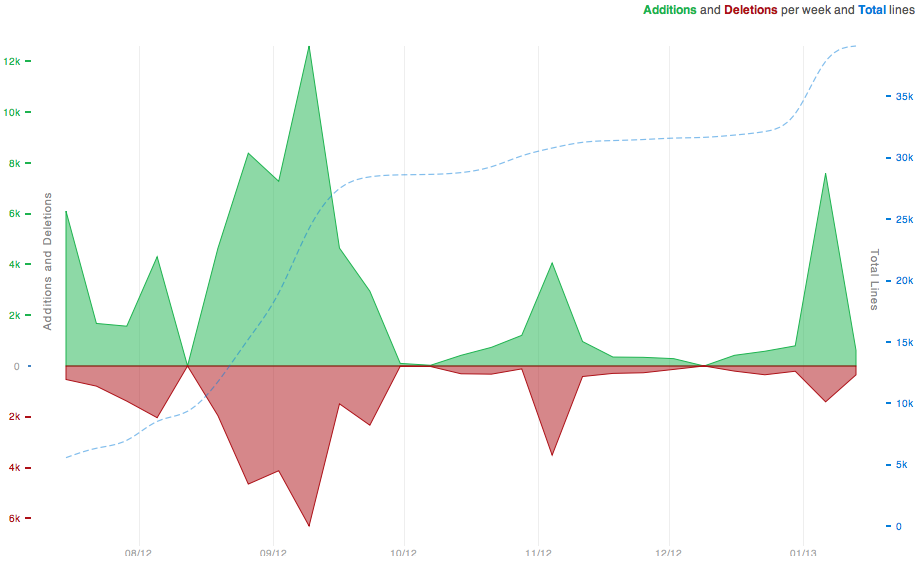
\includegraphics[scale=0.41]{pics/work.png}
\caption{Additions and deletions per week on GitHub}
\label{fig:GitHubGraphAddDel}
\end{center}
\end{figure}

\paragraph{Developing core components.}

%Summer 2012 – Development of the Concept, Include Parser, data structure for AST, BDD

After the formulation of the general concept with tutorials including 
exercises, a playground, a glossary, and the embedding of BoolTool,
the main classes for the representation of abstract syntax trees and binary decision diagrams were implemented.
After several failed attempts to cross-compile \verb=BoolTool='s sources \verb+OCaml+ 
and to use the binaries on iPad, the functionality of \verb+BoolTool+ was reimplemented as \BoolTool in Objective-C.
% A left recursive descendent parser for input strings with the syntax propositional logic was implement in Objective-C. 

\paragraph{Adding content, controllers, and configurations.}

Although the general concept was developed, content had to be expounded. 
The tutorials had to be written and the exercises had to be generated. 
Content and configuration files had to be added to the project. 
The different views had to be controlled and the navigation between the different use cases had to be added. 

\paragraph{Finishing.} In the final phase all parts of the program were reviewed.
\Nyaya's content was amended and this document was written. 
\Nyaya was prepared for distribution in the App Store.

\subsection{Development model}

The development of this software did no follow a specific development model, 
but did borrow some principles from agile development.

\paragraph{Fail-Fast.} The interaction with syntax trees and 
the integration of \verb=BoolTool= were identified as essential parts with a high risk potential. 
The first one was cleared by exploring the user interface capabilities.
The second one failed at the beginning of developing core components 
and was substituted with a native implementation of the functionality of \verb=BoolTool=
under direct control of the project.

\paragraph{Test-driven development.}

Parsers, trees and operations on trees were the ideal application for test driven development.
First, the expected results were defined in test cases, then the functionality was implemented.
So it was ensured that at every point of the development cycle 
the core of the application was still working as defined,
when all unit tests had succeeded.

\paragraph{Refactoring.}
Due to occurring memory and performance issues on the iPad
some implementations had to be reconsidered 
and some functionality had to be reimplemented.
This could be done without complications because 
the local repository provided a complete development history 
and unit tests provided a quick check, whether the reimplementation was correct.

\paragraph{Use cases.}
With the written concept (see chapter \vref{ch:concept}) of an interactive environment for BoolTool 
that enables the learning  of simple facts about propositional logic the collection of use cases was defined. 
These use cases represent the real value of the project 
and they mark the criterion for completion of development.

